\textit{ComplexOvercooked} is an open-source RL environment for all researchers for any non-commercial activity under the MIT License. In this section, we will introduce dynamic-objective challenges in this environment, order synthesis paths, and core elements (i.e., observation space, action space, and reward function setups) of RL agents. We provide three types of interfaces supporting RL agents, humans and LLMs. We emphasize the differences in these settings compared to that in original \textit{Overooked\_AI}.
\begin{figure}[htb]
    \centering
    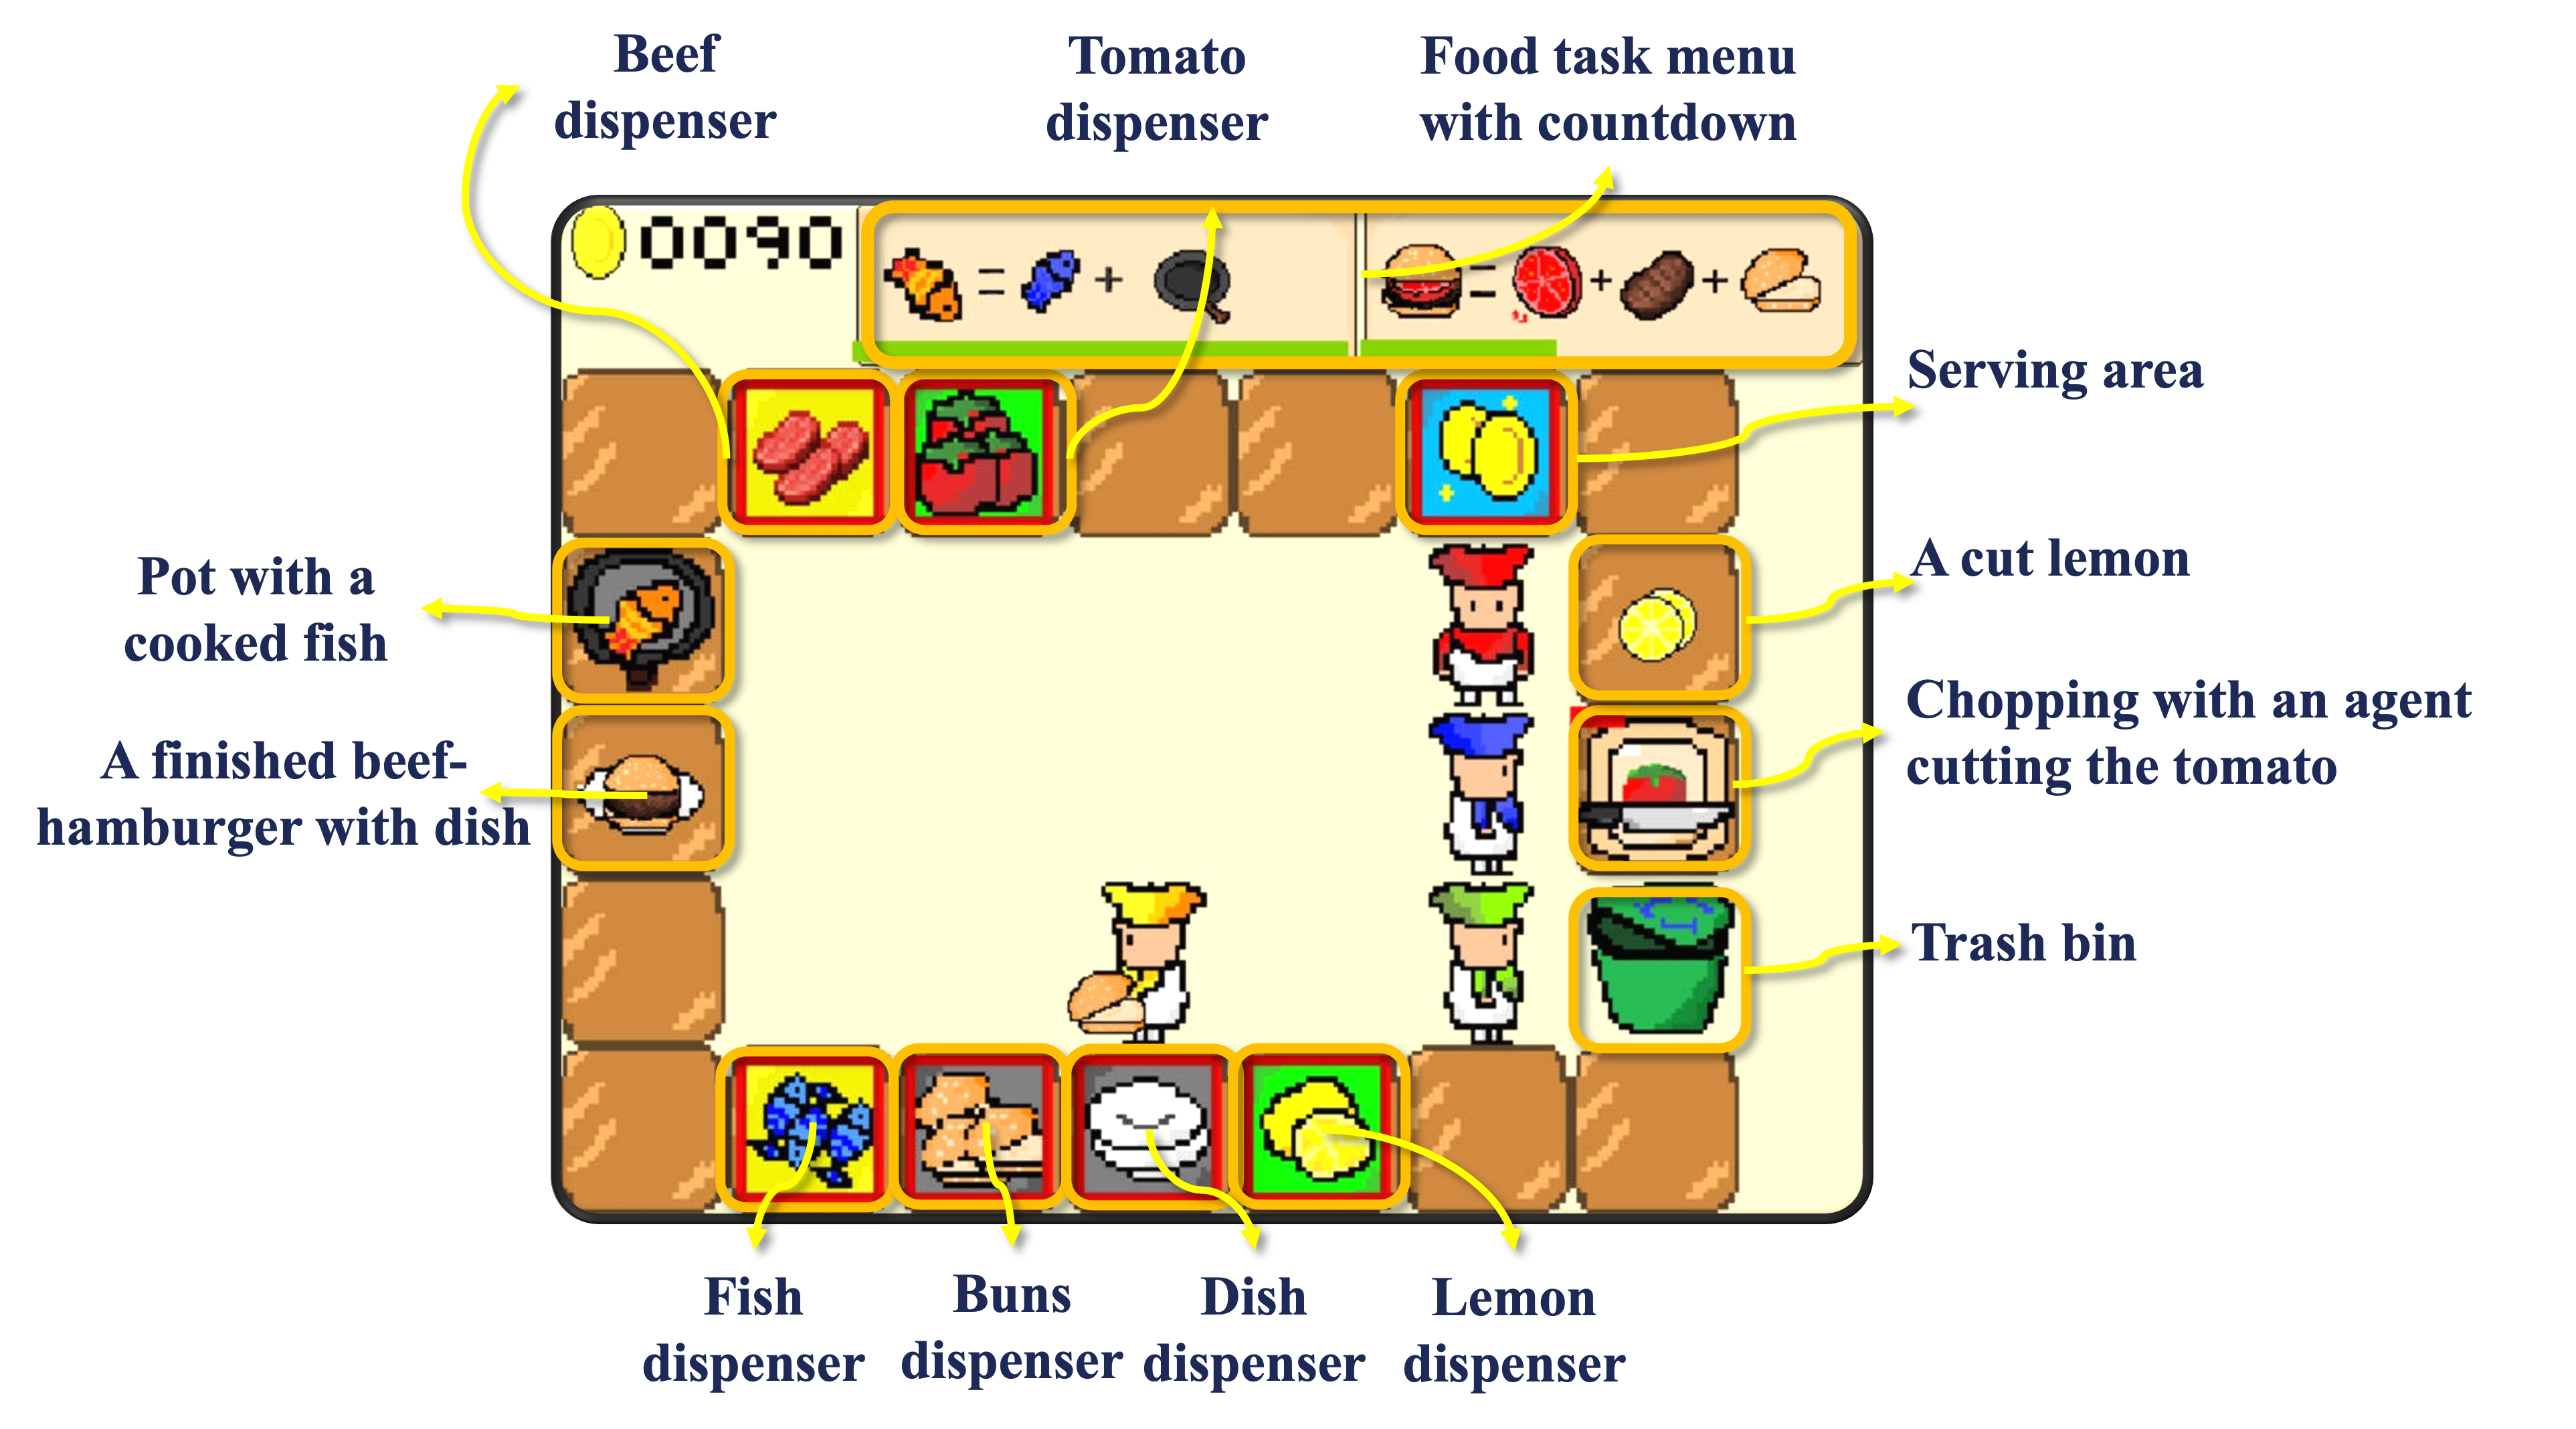
\includegraphics[width=\linewidth]{Figures/game_intro.png}
  \caption{The game interface of \textit{ComplexOvercooked}, in which multiple orders are generated randomly and they need to be finished simultaneously as listed in the task menu.}
\label{fig:intro}
\end{figure}
\subsection{Dynamic-objective challenge}
In the Overcooked game, players need to cook specific dishes based on user orders (shown at the top of Figure \ref{fig:intro}). Different orders are randomly generated and have distinct synthesis paths (Figure \ref{fig:recipe}), which determine whether the user's current actions will receive rewards. In the default game configuration, each order lasts for 200 time steps, and users must complete the cooking within this time frame. Failing to deliver the order within the time limit results in no reward or even a penalty. This dynamic objective poses a significant challenge for multi-agent training.

In the current game, we provide four types of orders: \textit{Cookedfish}, \textit{Cookedbeefhamburger}, \textit{AClemoncookedfish} and \textit{ACtomatocookedbeefhambuger}. These orders vary in difficulty and reward. For example, the steps required for \textit{AClemoncookedfish} are: cook fish using a pot, cut lemon using a cutting table and combine the cooked fish and cut lemon,  while \textit{Cookedfish} is much simpler, requiring only placing raw fish into the pot, waiting for a certain time, and then serving it on a plate. Higher-difficulty orders take more time to complete but yield greater rewards, forcing agents to make trade-offs during training.
\begin{figure}[H]
    \centering
    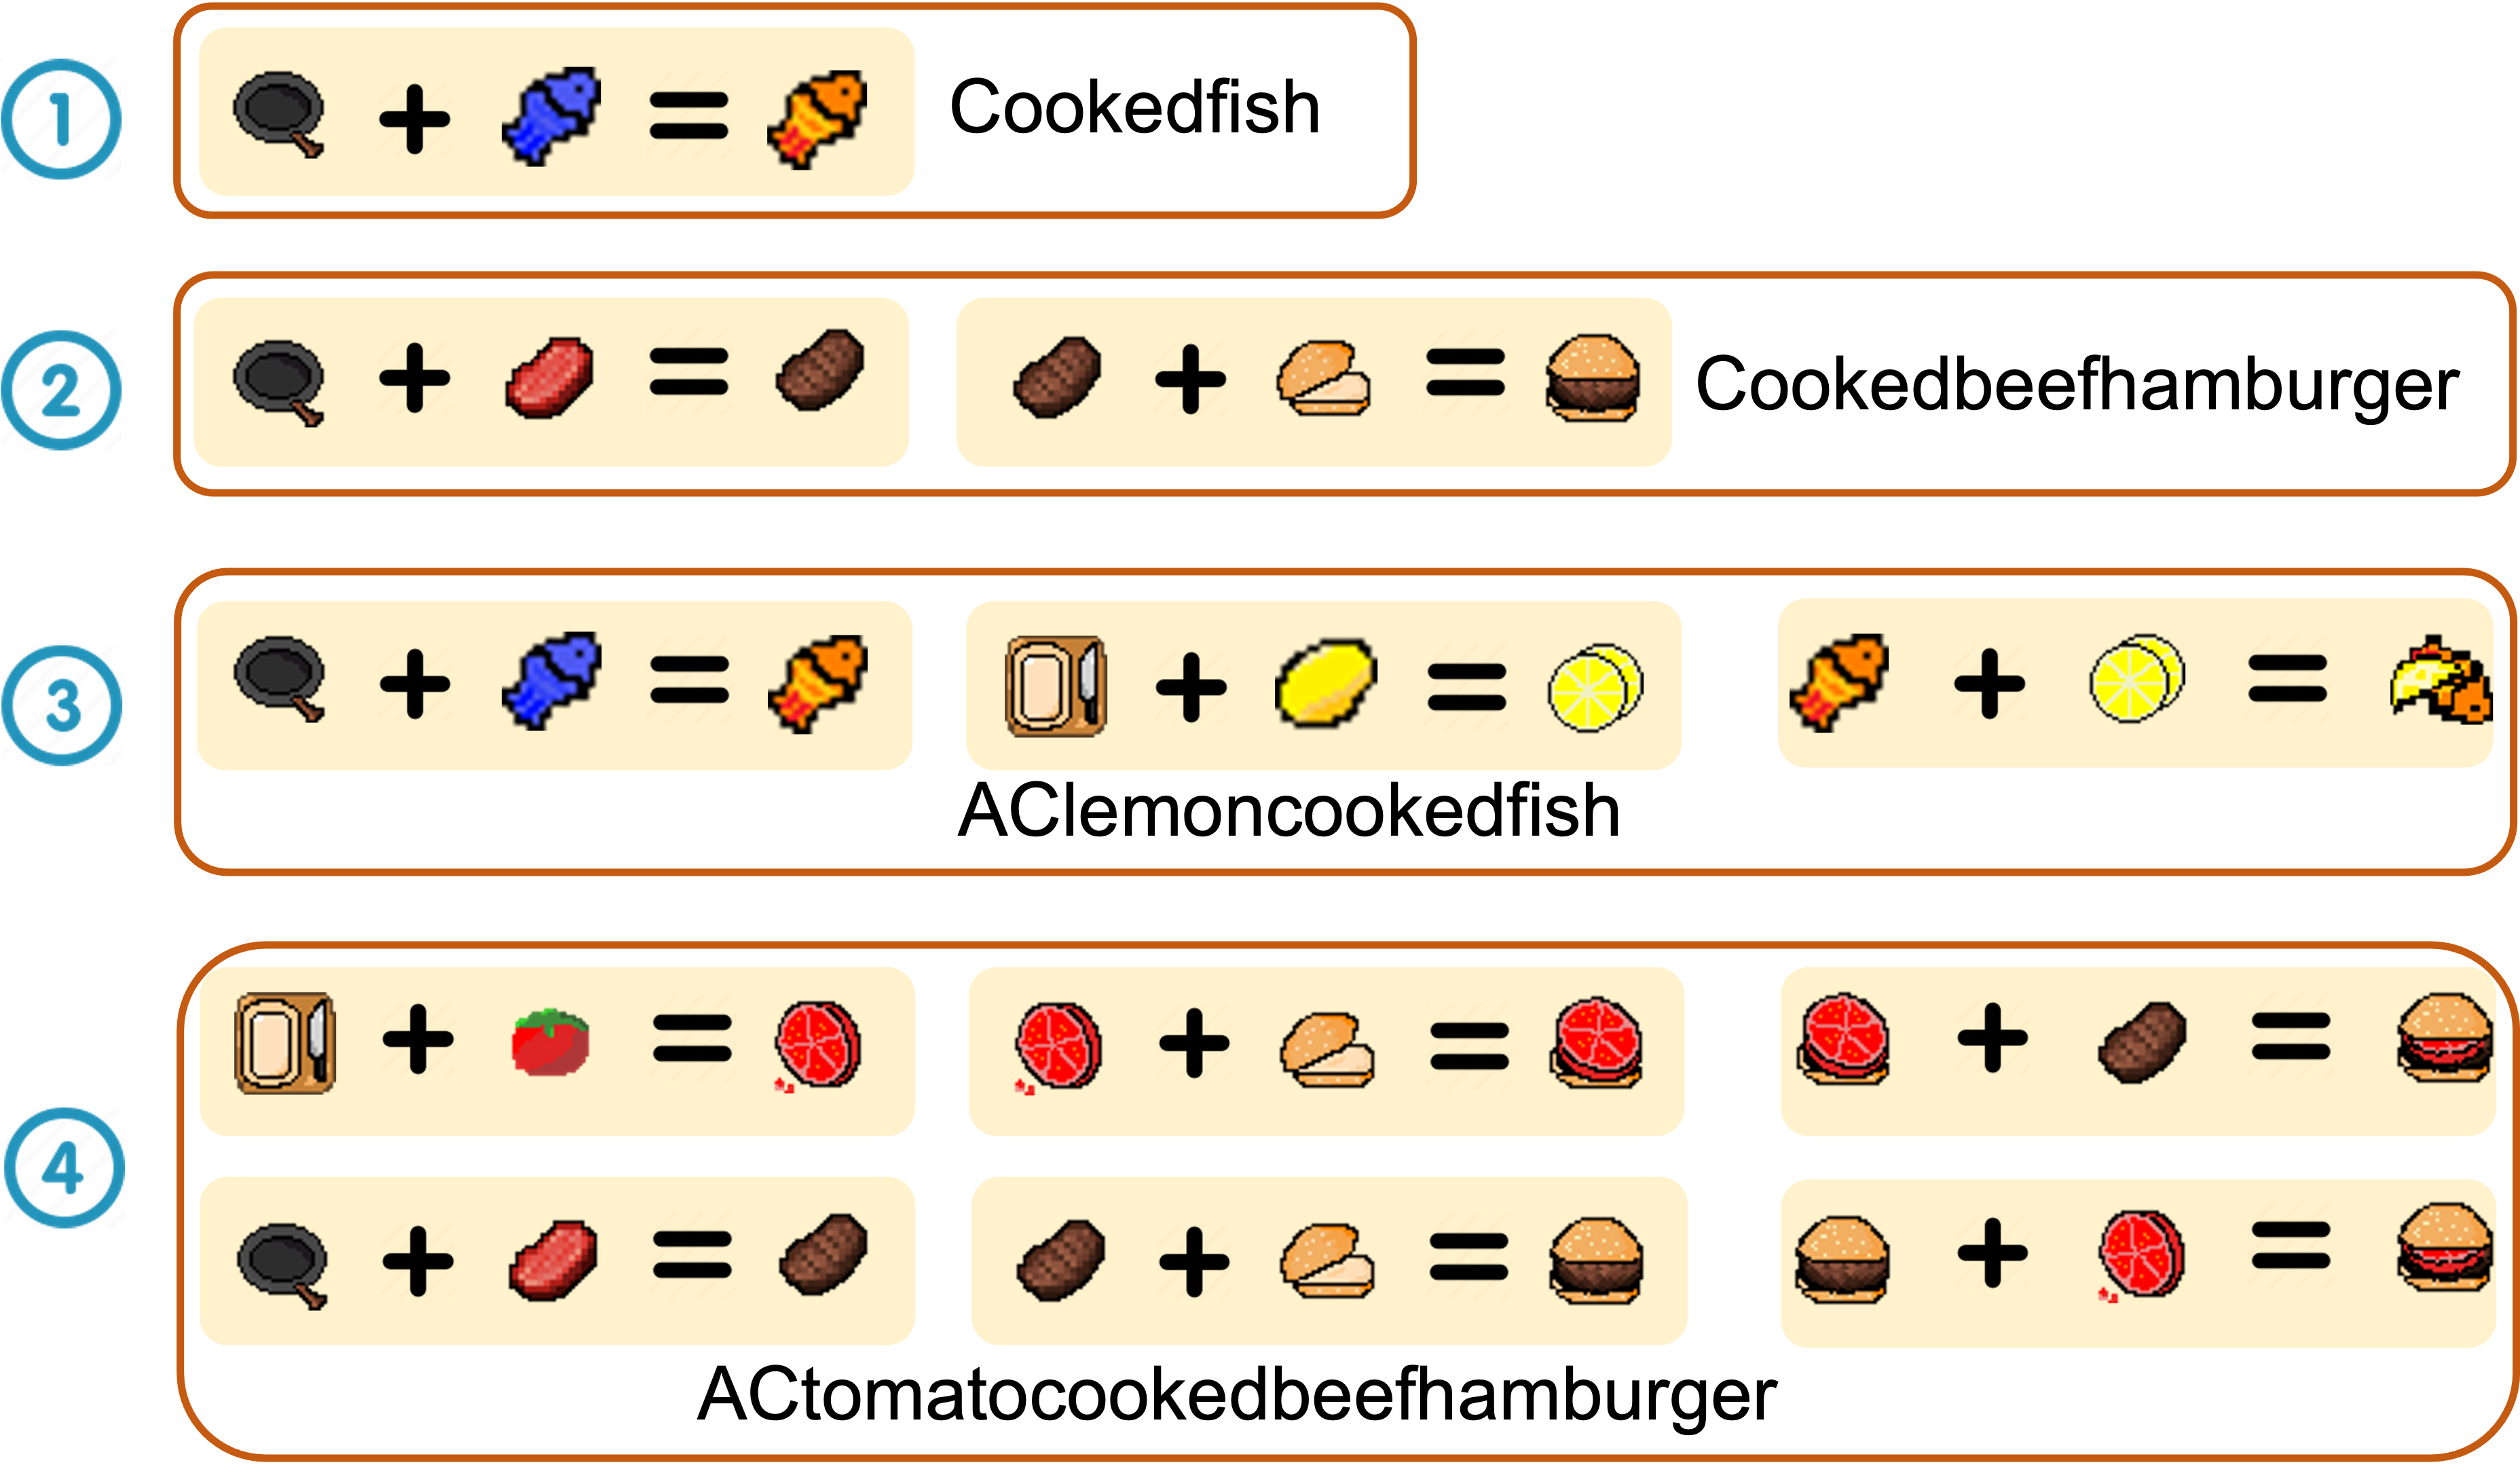
\includegraphics[width=\linewidth]{Figures/recipe.png}
  \caption{Recipes and synthesis paths of orders in \textit{ComplexOvercooked}}
\label{fig:recipe}
\end{figure}

\subsection{Control interfaces}
To empower research in the field of collaboration among agents, LLMs, and humans, we provide three types of control interfaces to facilitate the study of subsequent control algorithms.\\
\textbf{Human} \ Human players can control the actions of the chef in the game via the keyboard and can set one of the chefs as an AI to conduct a human-AI cooperation. In addition, the trajectories of human players can be easily collected for imitation learning. \\
\textbf{RL agent} \ Based on observations of the environment, RL agent can decide on a sequence of actions that maximize its episodic reward. We provide several MARL algorithms for researchers in this work. \\
\textbf{LLM agent} \ To explore the combination of LLM with  RL agents and humans, we offer semantic presentations of the environment, enabling these models to understand the game rules, current state, and agents' objective, to recommend appropriate actions to complete orders.\\
\subsection{Agents}
We provide a general description of the following core elements of RL agents, among which observation space, reward ffunction,and episode dynamics can be configured in the game settings. \\
\textbf{Observation space} \  \textit{ComplexOvercooked} is a fully observable environment. We provide two choices (\textit{flattened vector} and \textit{multi-channel matrix}) to encode the global state. Flattened vector includes the ego agent and partners' features, the relative position of the agent with each partner, the agents' absolute position, and task-related features. The agent's own feature includes its facing direction, held item, whether it is cutting, whether it is blocked by the wall, and the relative distance to each functional entity (e.g., the pot, the dish dispenser and the cutting board). The relative positions of the ego agent with its partners are represented as coordinates \texttt{(dx, dy)}. Task-related features include the current game duration, order type, etc. The observation space of the agent can be taken using the \texttt{get\_obs()} function, and it varies according to the number of agents and functional entities. Compared to \textit{Overcooked\_AI}, we add many functional entities and use task-related features, which make the observation space larger. Multi-channel matrix with dimension \texttt{(layout height,layout width,n\_channels)} uses one channel to represent one feature. For example, one channel with \texttt{True} value in it can represent the corresponding position: is a pot/cutting table or the pot/cutting table is ready.   \\
\textbf{Action space} \ The agent's action space is discrete and includes moving up, down, left, right, staying, or interacting with the entity in front.\\
\textbf{Reward setups} \ In Overcooked game, the final score depends on how many orders are completed in a limited time. Due to the high complexity of the game and the large state space, the rewards for completing orders (Table \ref{tab:sparse reward}) are relatively sparse for agents. To ensure the convergence of MARL algorithms, we introduce more shaped rewards, as shown in Table \ref{tab:shaped reward}.

\begin{table}[htb]
\centering
\caption{Sparse reward setups}
\label{tab:sparse reward}
\setlength{\tabcolsep}{3.5mm}
\begin{tabular}{lc}
\toprule
\textbf{Sparse reward} & \textbf{Value} \\
\midrule
AClemoncookedfish  & 20         \\
Cookedfish    & 10    \\
ACtomatocookedbeefhamburger  & 25  \\
Cookedbeefhamburger        & 15     \\
\bottomrule
\end{tabular}
\end{table}

\begin{table}[htb]
\centering
\caption{Shaped reward setups}
\label{tab:shaped reward}
\setlength{\tabcolsep}{3.5mm}
\begin{tabular}{lc}
\toprule
\textbf{Shaped reward} & \textbf{Value} \\
\midrule
Get need cutting  & 3    \\
Get need cooking  & 3    \\
Synthesis of AClemoncookedfish & 5  \\
Synthesis of Cookedfish & 2  \\
Synthesis of ACtomatocookedbeefhamburger & 6  \\
Synthesis of Cookedbeefhamburger        & 3     \\
\bottomrule
\end{tabular}
\end{table}

% Agents only receive a sparse reward when they deliver a dish that is on the task menu. Delivering dishes not on the menu or failing to deliver within the time limit will not yield any sparse rewards. To train the agents, we have designed additional configurable shaped rewards including: pick dish, pick need material, synthesis, cutting, get need cutting, cooking, get need cooking, synthesizing new food, carrying using dish. The rewards comprise of  The one-step reward of the agent that can be take using the \texttt{calculate\_rew()} function. Compared to original \textit{Overcooked}, it is much more difficult to obtain the final reward, so we designed detailed shaped rewards to facilitate the training of agents. 